

 %Pre-amble

\documentclass{beamer}
\usepackage{beamerthemeshadow}
\usepackage{graphicx}
\graphicspath{ {images/} }
\begin{document}
\title{Grammar of Graphics}  
\author{Brian Perron, Ph.D.}
\date{\today} 

\begin{frame}
\titlepage
	\begin{center}
		\includegraphics[width=40mm,scale=0.5]{datalab.png}
	\end{center}
\end{frame}

\begin{frame}\frametitle{Key points}
\tableofcontents[hideallsubsections]
\end{frame} 





%%%%%%%%%%%%%%%%%%%%%%%%%%%%%%%%%%%%%%%%%%
%                                   Overview of the grammar                					 %
%%%%%%%%%%%%%%%%%%%%%%%%%%%%%%%%%%%%%%%%%%

\section[Overview of the grammar]{Conceptual overview of the grammar of graphics}
\subsection{Original}

\begin{frame}
\begin{center}
Conceptual overview of the grammar of graphics
\end{center}
\end{frame}

\frame{\frametitle{The original grammar}
\framesubtitle{Leland Wilkinson}
	\begin{columns}
		\begin{column}{5cm}
			\begin{itemize}
				\item \footnotesize{Bertin's Semiology of Graphics (1967) }
				\item Graphics Production Library (GPL)
				\item SYSTAT, SPSS, Tableau
			\end{itemize}
		\end{column}
	\begin{column}{5cm}
		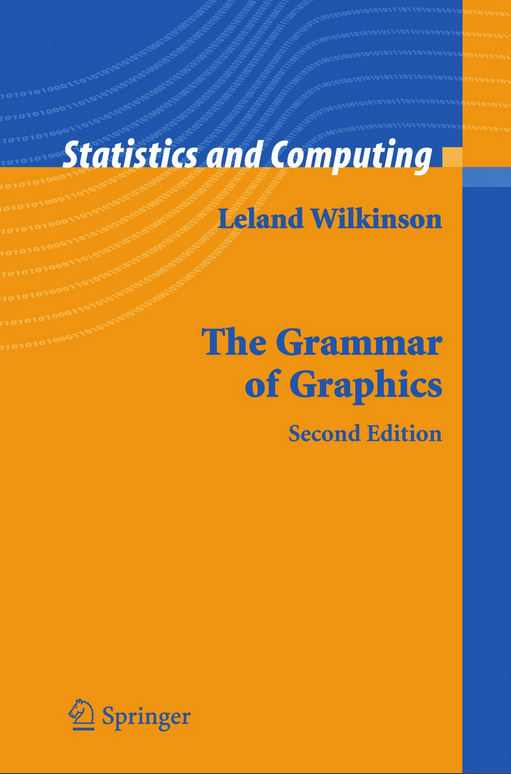
\includegraphics[width=40mm,scale=0.5]{gog.png}
		\end{column}
	\end{columns}
}


\begin{frame}\frametitle{Motivations for a grammar}
	\begin{itemize}
		\item To describe deep features that underlie all graphics
		\item Provides language-based rules
		\item Beyond chart typologies to unlimited graphical forms 
		\item Emphasis on effective display of data 
	\end{itemize}
\end{frame}



\begin{frame}\frametitle{The graphical pipeline}
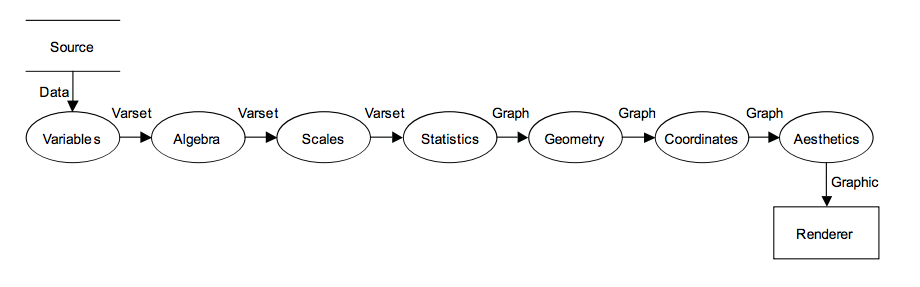
\includegraphics[width=110mm]{originalframework.png}
\end{frame}



\subsection{Revisioned}

\frame{\frametitle{The grammar revisioned}
	\begin{columns}
		\begin{column}{5cm}
			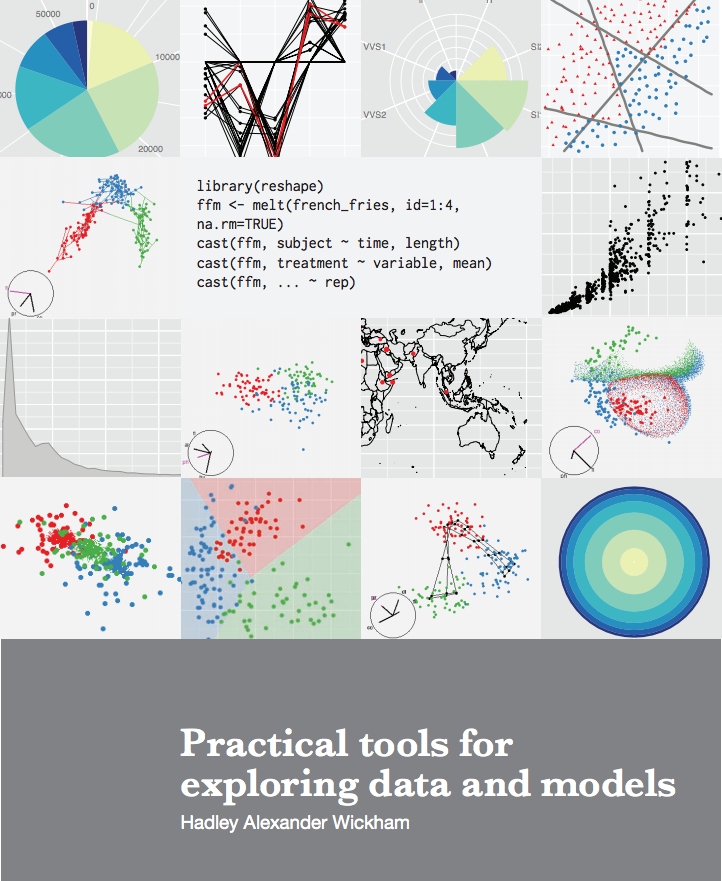
\includegraphics[width=40mm,scale=0.5]{dissertation.png}
			
		\end{column}
	\begin{column}{5cm}
		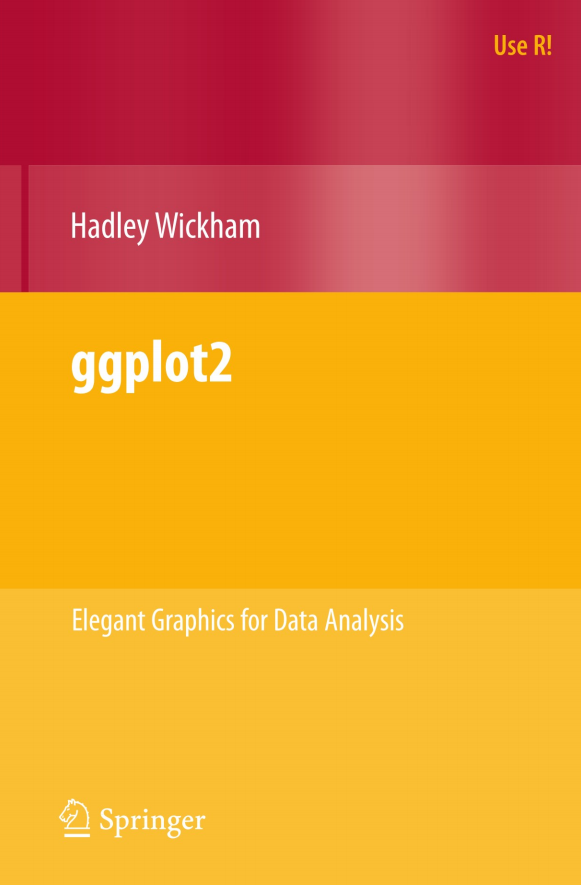
\includegraphics[width=40mm,scale=0.5]{ggplot2.png}
		\end{column}
	\end{columns}
}

\begin{frame}\frametitle{The grammar revisioned}
\begin{block}{What is maintained?}
	\begin{itemize}
		\item Original graphical language
		\item Conceptual framework of graphics
		\item Motivations for describing deep structure
	\end{itemize}
\end{block}

\medskip

\begin{alertblock}{What is different?}
	\begin{itemize}
	\item Primacy on layered development
	\item Graphical pipeline
	\end{itemize}
\end{alertblock}
\end{frame}

\subsection{ggplot2}

\begin{frame}\frametitle{Plotting functions}
\begin{alertblock}{qplot}
	\begin{itemize}
		\item Quick plot 
		\item Similar to \texttt{plot} in base R
		\item Rapid exploration of data
		\item Limited use of the grammar
	\end{itemize}
\end{alertblock}

\begin{exampleblock}{ggplot}
	\begin{itemize}
		\item Infinite number of graphical options
		\item Full control over the grammar
		\item Extensible
		\item Limited scalability
	\end{itemize}
\end{exampleblock}
\end{frame}

\begin{frame}\frametitle{qplot vs. ggplot}
\framesubtitle{Minimal example}

\footnotesize\texttt{p <- qplot(data=diamonds, carat, price)}

\bigskip 

\footnotesize\texttt{p <- ggplot(data=diamonds, aes(carat, price)) + geom\_point()} 
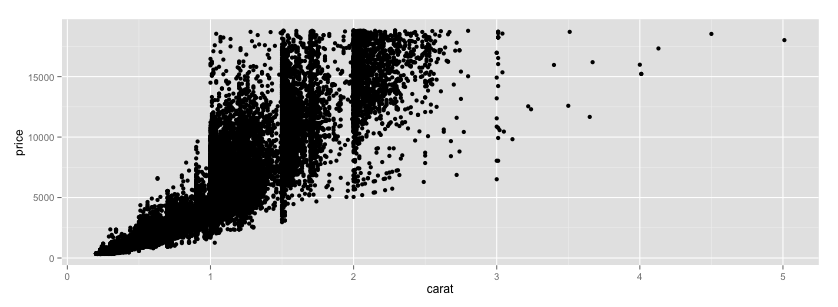
\includegraphics[width=100mm,scale=0.5]{qplotbw.png}
\end{frame}

%%%%%%%%%%%%%%%%%%%%%%%%%%%%%%%%%%%%%%%%%%
%                                Essential elements                        			                        %
%%%%%%%%%%%%%%%%%%%%%%%%%%%%%%%%%%%%%%%%%%

\section[Essential elements of the language]{Essential elements of the graphical language}

\begin{frame}
\begin{center}
Essential elements of the graphical language
\end{center}
\end{frame}

\begin{frame}\frametitle{Graphical language}
\framesubtitle{Parts of speech}
	\begin{enumerate}
	\item \alert{Data} (variables and algebra)
	\item Transformations (linear, log)
	\item \alert{Geometry} 
	\item Scales (\alert{aesthetics})
	\item Statistics (summarized vs. unsummarized data)
	\item Coordinate system (cartesian, polar, \texttt{facet})
	\item Guides (axes, legends, annotations, etc.)
	\end{enumerate}
\end{frame}

\subsection{Geometry}
\begin{frame}\frametitle{Geometry}
\framesubtitle{Graphical language}
	\begin{alertblock}{geom}
	\begin{itemize}
		\item Things that you see
		\item Lines, points, bars, polygons, area, etc.
		\item Defines the range of aesthetic attributes
		\item Constitutes a single layer
		\item Each unique layer contains a data set
		\item Painter's model
	\end{itemize}
	\end{alertblock}
	\end{frame}

\subsection{Aesthetics}
\begin{frame}\frametitle{Aesthetics}
\framesubtitle{Graphical language}
	\begin{exampleblock}{aes}
		\begin{itemize}
			\item \alert{Mapping} of aesthetic properties to a layer 
			\item Position within coordinate system
			\item Attributes of geometry 
			\item Color, shape, size, group
		\end{itemize}
	\end{exampleblock}
\end{frame}

\subsection{Data}
\begin{frame}\frametitle{Data}
\framesubtitle{Graphical language}
	\begin{block}{data}
		\begin{itemize}
			\item Derive variables from the data
			\item Each aesthetic must have a variable mapping
			\item Each geometry has a corresponding dataframe
			\item Data must be an R dataframe
			\item Variable(s) for faceting
			\item Summarized versus unsummarized data (\texttt{stat})
		\end{itemize}
	\end{block}
	\bigskip

\begin{center}

I 
\includegraphics[width=6mm,scale=0.5]{heart.png} melted data \ldots

\end{center}

\end{frame}

%%%%%%%%%%%%%%%%%%%%%%%%%%%%%%%%%%%%%%%%%%
%                                Application to the workflow                     			              %
%%%%%%%%%%%%%%%%%%%%%%%%%%%%%%%%%%%%%%%%%%

\section{Grammar applied to the workflow}

\begin{frame}
\begin{center}
Grammar applied to the workflow
\end{center}
\end{frame}

\subsection{Old workflow}
\begin{frame}\frametitle{The old way of working}
\begin{enumerate}
	\footnotesize
	\item Have idea 
	\item Start hacking 
	\item Google search \
	\item Swear, get coffee, and return to hacking 
	\item Search StackOverflow
	\item Everything but one thing working 
	\item Swear, get coffee, and return to hacking
	\item Swear
	\item Post on StackOverflow 
	\item Post closed, redirected to unhelpful post
	\item Hacking finally works but not sure why 
	\item Mediocre graphic \ldots \alert{repeat workflow}
\end{enumerate}
\end{frame}

\subsection{New workflow}
\begin{frame}\frametitle{Where to begin?}
\framesubtitle{Example workflow}


\begin{enumerate}
	\item Establish the storyline 
	\item Determine best way to visually encode 
	\item Design the graphic (outside of R) 
	\item Describe the graphic with the grammar 
	\item Shape the data 
	\item Execute in \texttt{ggplot} 
	\item Tufte-fy 
\end{enumerate}
\end{frame}

\subsection{Encoding \& decoding principles}

\begin{frame}\frametitle{Visual encoding \& decoding principles}
\framesubtitle{Theory of Graphical Perception - Cleveland \& McGill}
\begin{center}
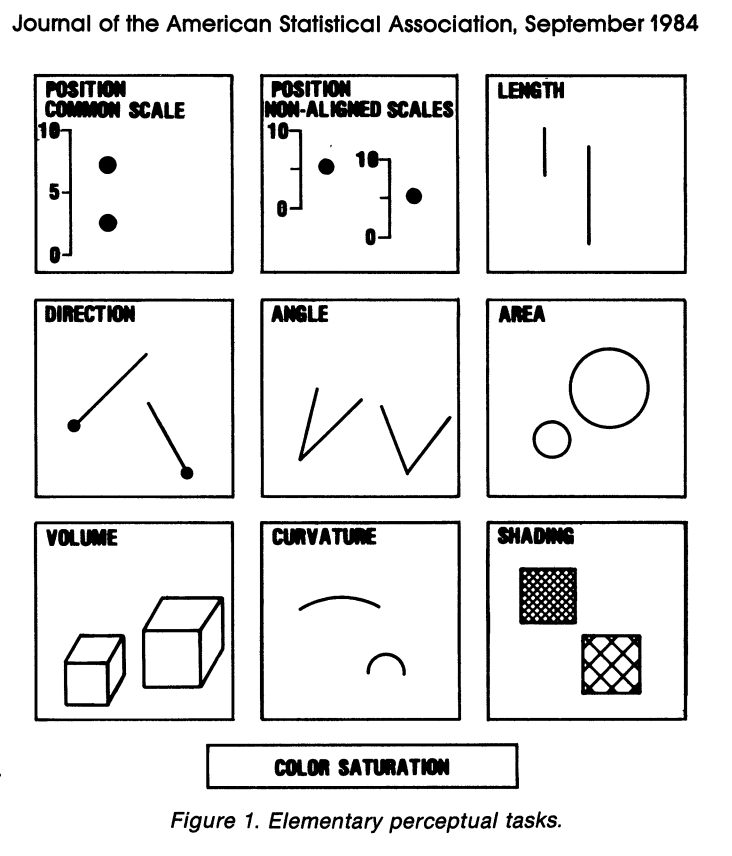
\includegraphics[width=60mm,scale=0.5]{cleveland.png}
\end{center}
\end{frame}


\begin{frame}\frametitle{Visual encoding \& decoding principles}
\framesubtitle{Pre-attentive processing}
\begin{center}
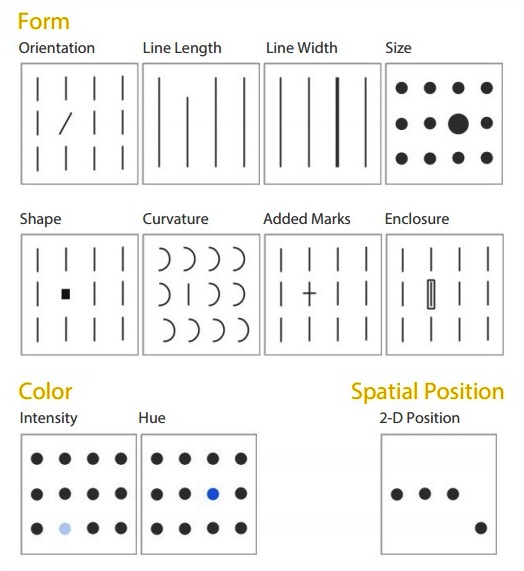
\includegraphics[width=50mm,scale=0.5]{colinware.jpg}
\end{center}
\tiny{Image credit:  Colin Ware, Information Visualization: Perception for Design}
\end{frame}


\begin{frame}\frametitle{Visual encoding \& decoding principles}
\framesubtitle{Analytic patterns from attributes}
\begin{center}
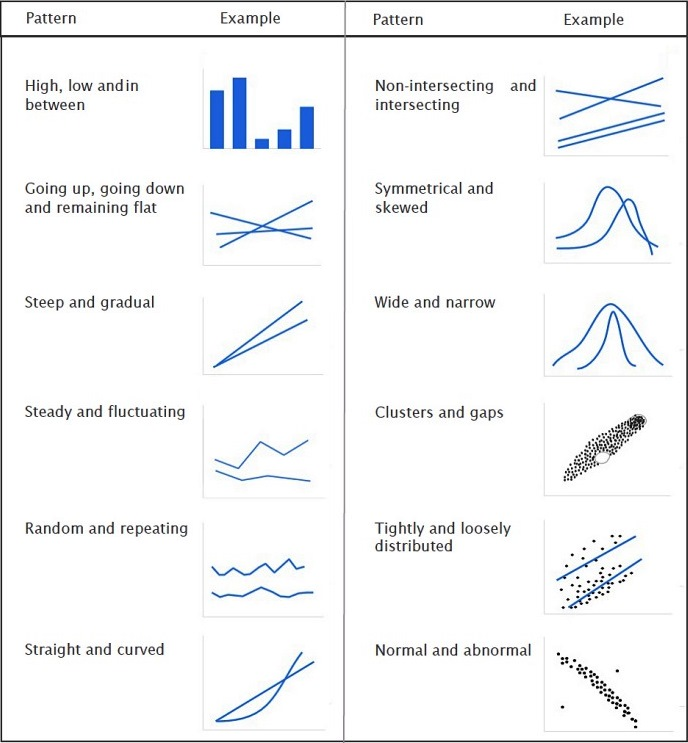
\includegraphics[width=50mm,scale=0.5]{few.jpg}
\end{center}
\tiny{Image credit:  Stephen Few, Now you see it: Simple visualization techniques for quantitative analysis}
\end{frame}

\subsection{Design \& describe}
\frame{\frametitle{Design your graphic}
\framesubtitle{Analog approach}
	\begin{columns}
		\begin{column}{5cm}
			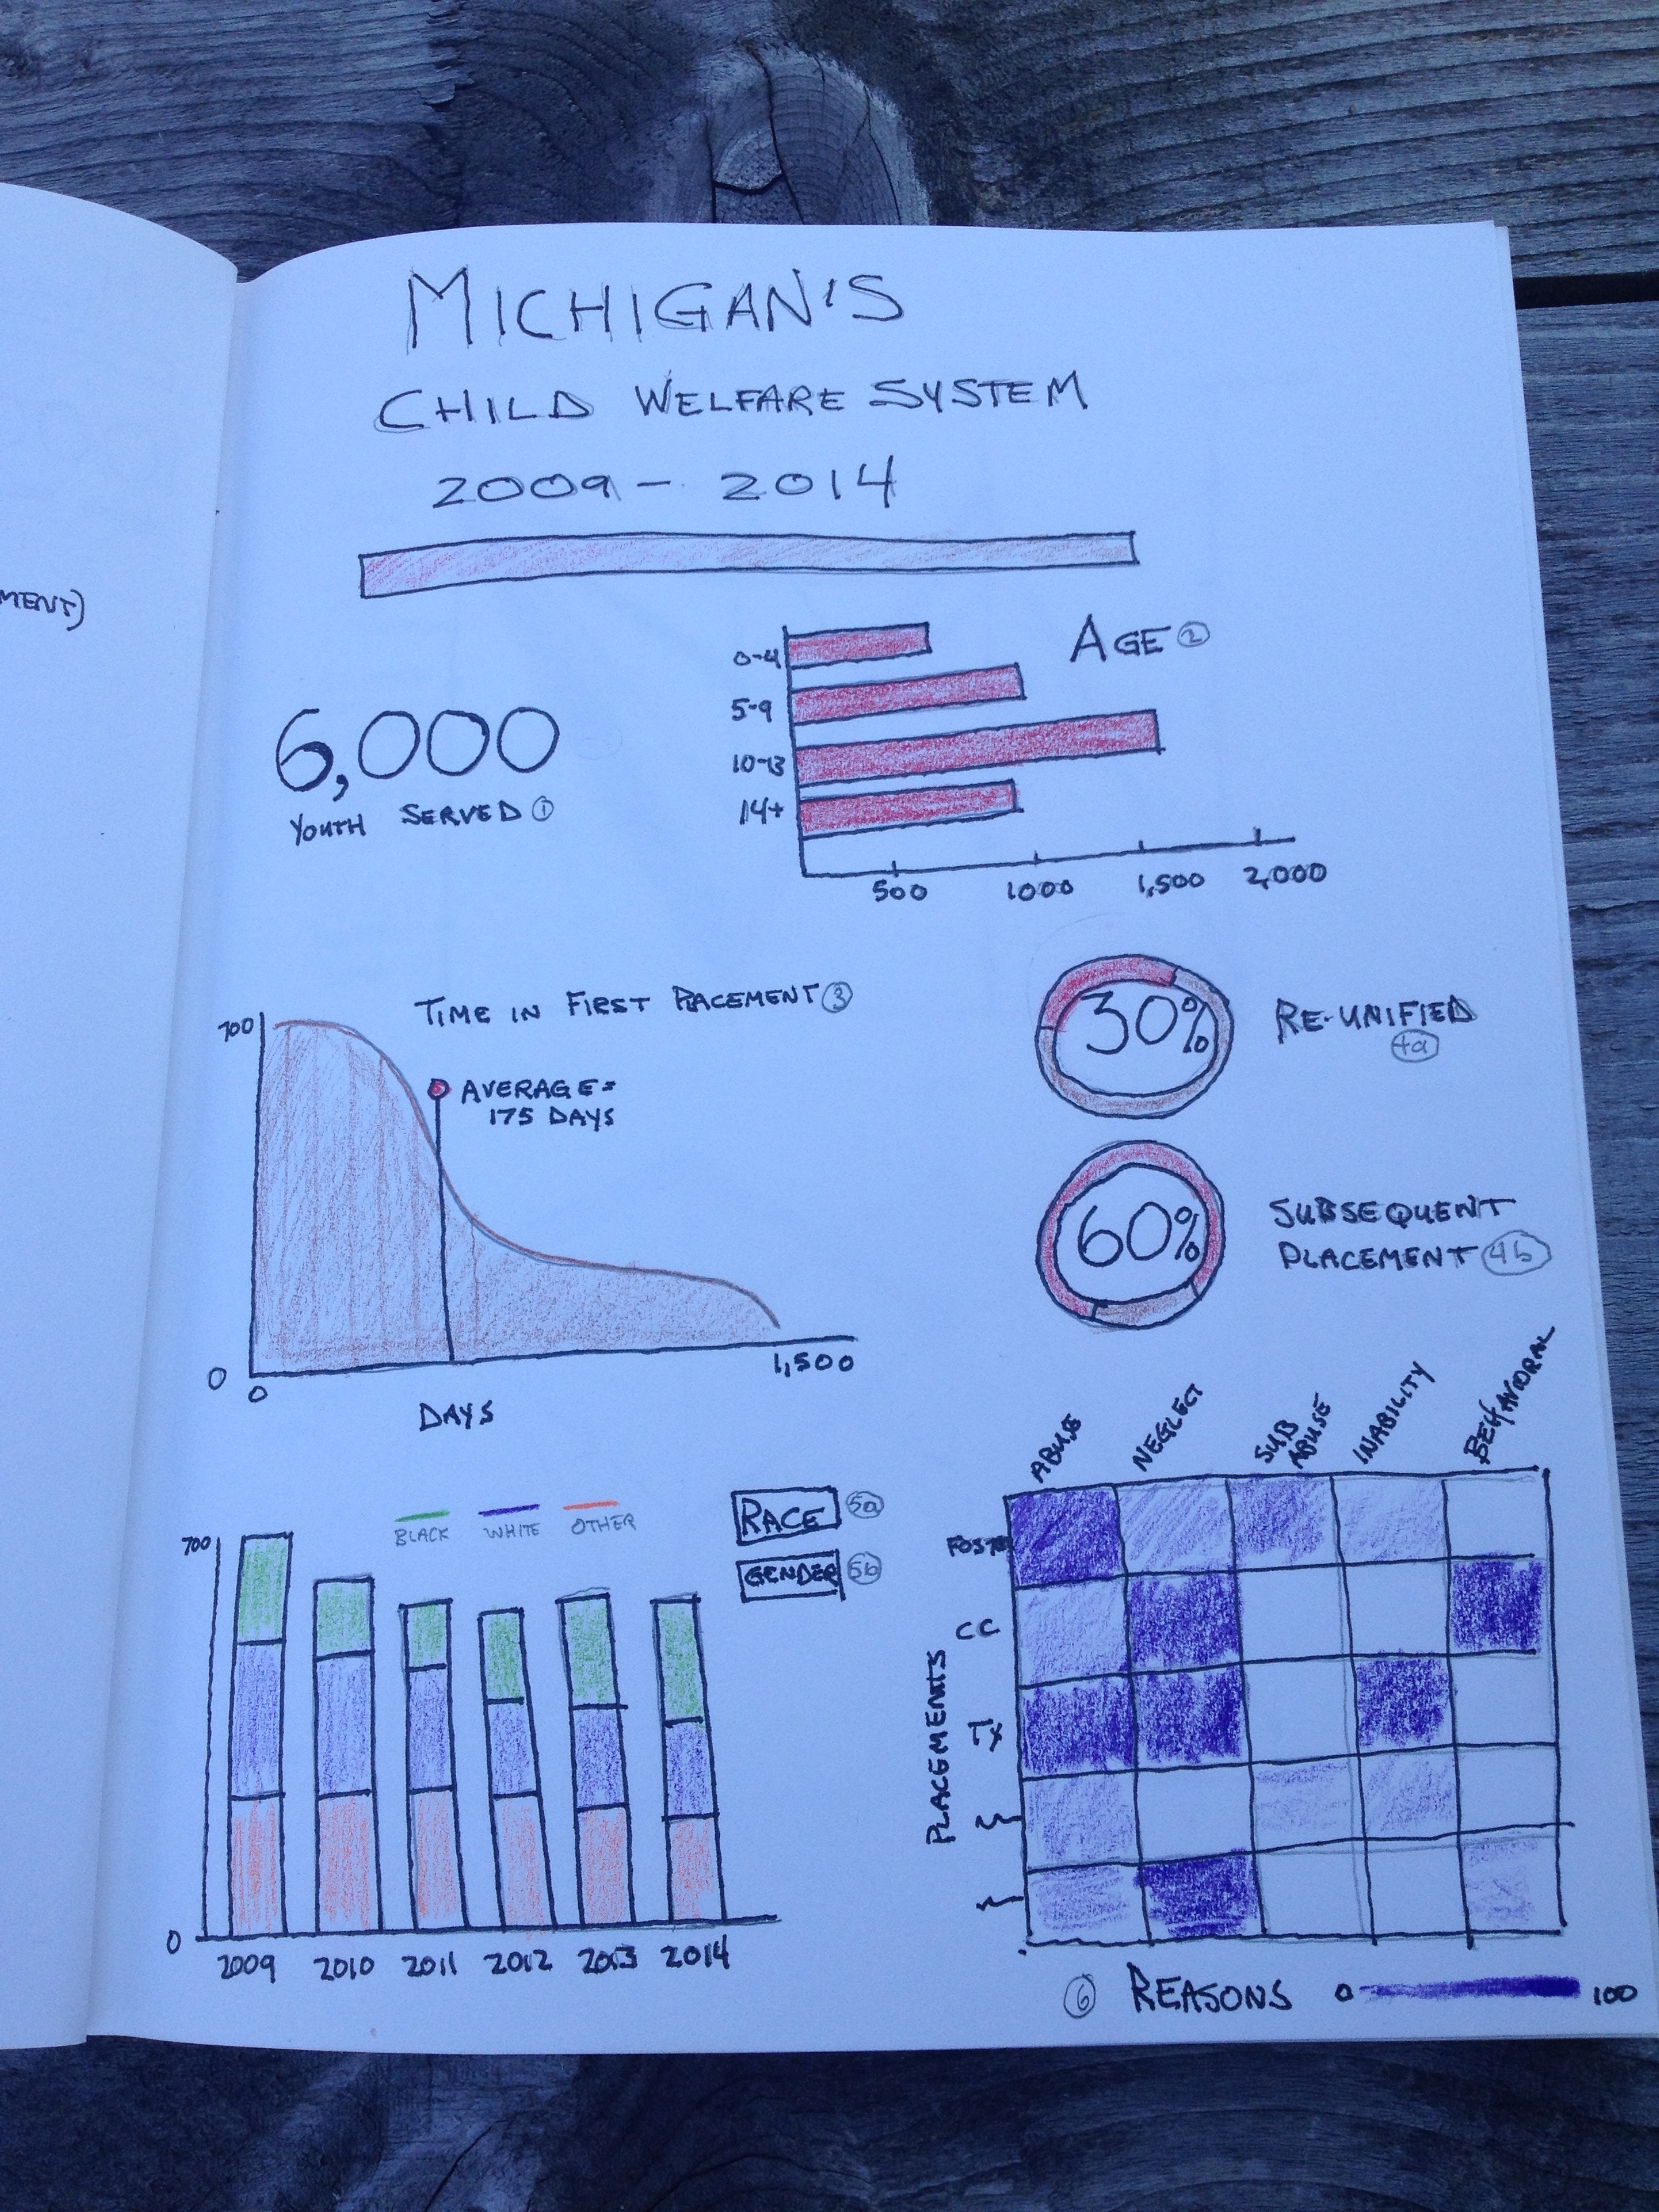
\includegraphics[width=40mm,scale=0.5]{analog2.jpg}
			
		\end{column}
	\begin{column}{5cm}
		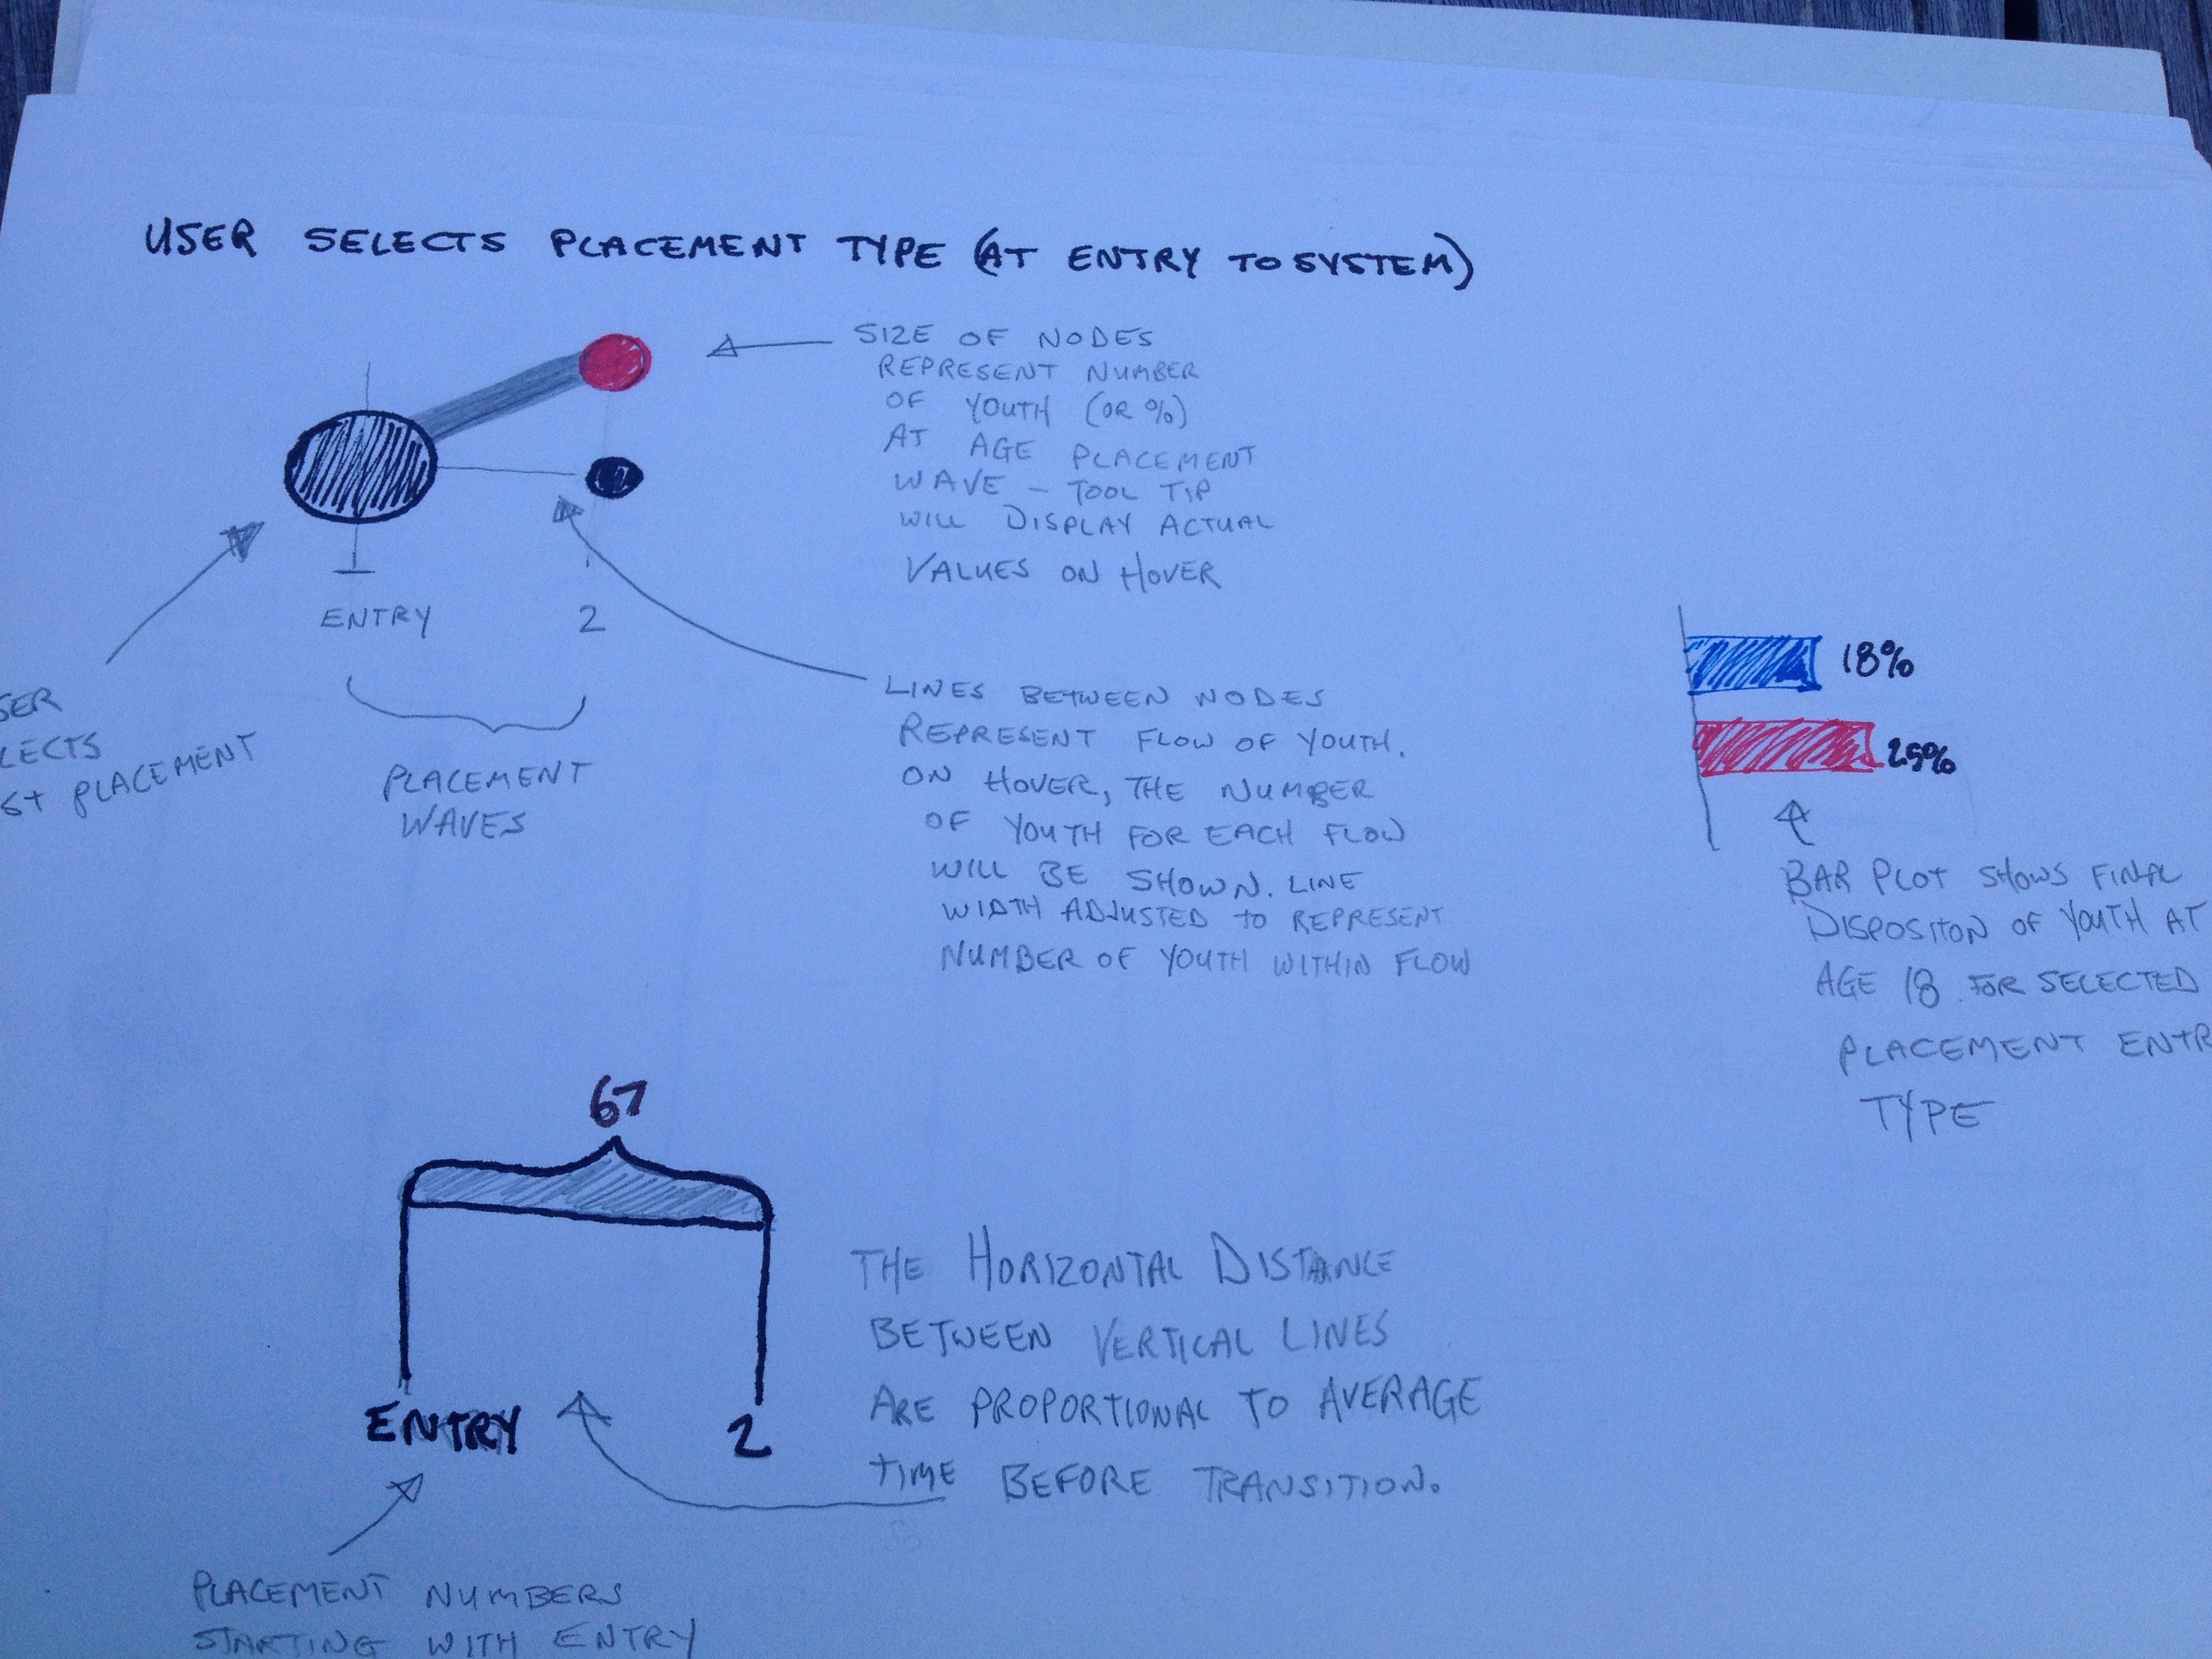
\includegraphics[width=40mm,scale=0.5]{analog1.jpg}
		\end{column}
	\end{columns}
}


\begin{frame}\frametitle{Describe the graphic with the grammar}
\framesubtitle{Applying the graphical language}
	\begin{itemize}	
	\item \alert{Data} 
	\item Transformations (outside of ggplot if possible)
	\item \alert{Geometry} 
	\item \alert{Scales \& aesthetics}
	\item Statistics (summarized vs. unsummarized data)
	\item \alert{Coordinate system} (facet)
	\item Guides (Final touches)
	\end{itemize}
\end{frame}
		

\section{Relate graphical language to code}

\begin{frame}
\begin{center}
Relate graphical language to code
\end{center}
\end{frame}

\begin{frame}\frametitle{Remember that ugly scatterplot?}
\footnotesize\texttt{p <- ggplot(data=diamonds, aes(carat, price)) + geom\_point()} 
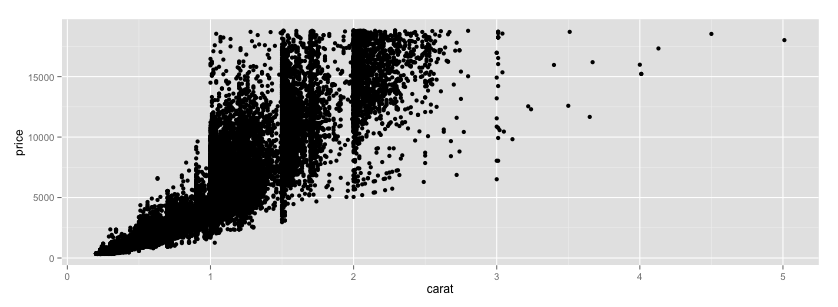
\includegraphics[width=100mm,scale=0.5]{qplotbw.png}
\end{frame}


\begin{frame}\frametitle{Remember that ugly scatterplot?}
\footnotesize\texttt{p <- ggplot(data=diamonds, aes(carat, price, colour = clarity)) + geom\_point()} 
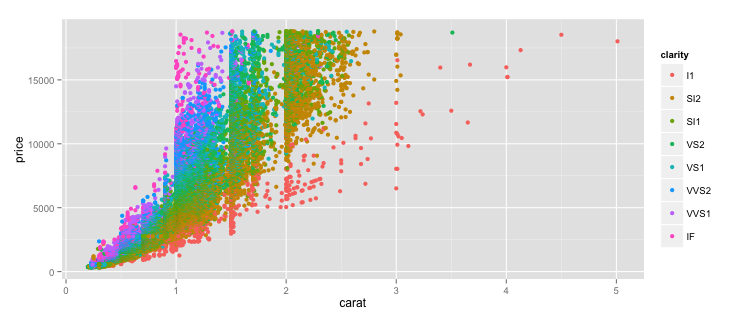
\includegraphics[width=100mm,scale=0.5]{qplot.png}
\end{frame}

\begin{frame}\frametitle{Under the hood}
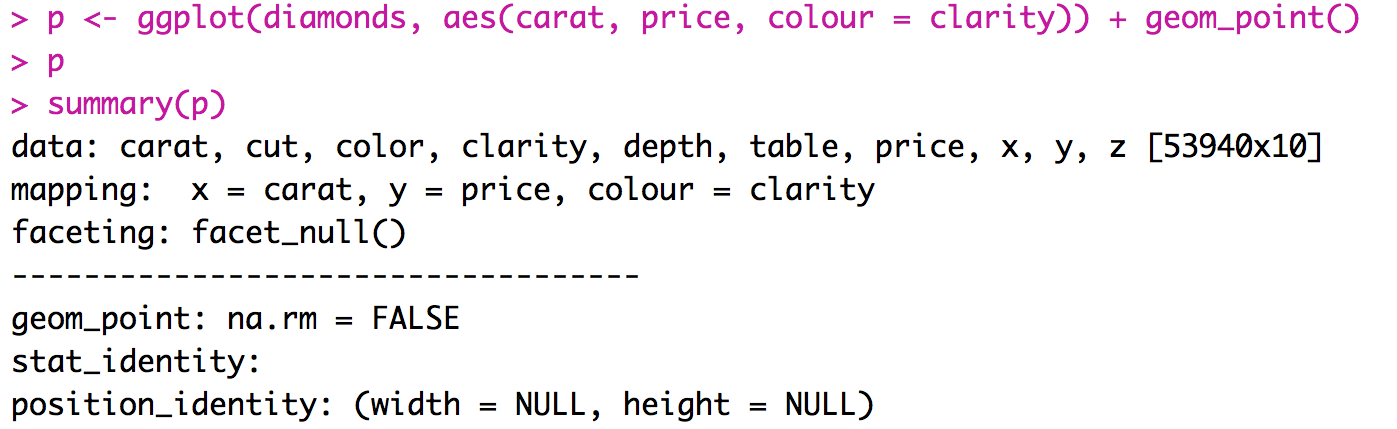
\includegraphics[width=110mm,scale=0.5]{hood.png}
\end{frame}


\begin{frame}\frametitle{How about blue points?}
\footnotesize\texttt{p <- ggplot(data=diamonds, aes(carat, price, colour = "blue")) + geom\_point()} 
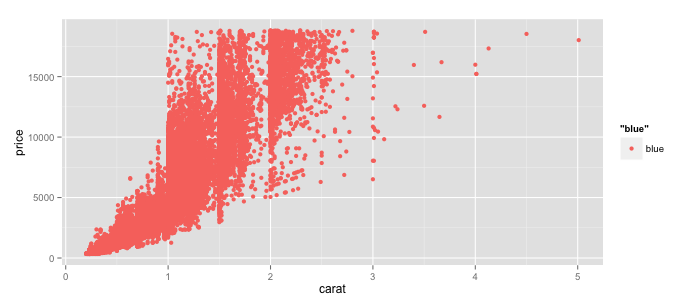
\includegraphics[width=100mm,scale=0.5]{qplotblue.png}
\alert{WTF?}
\end{frame}

\begin{frame}\frametitle{Under the hood}
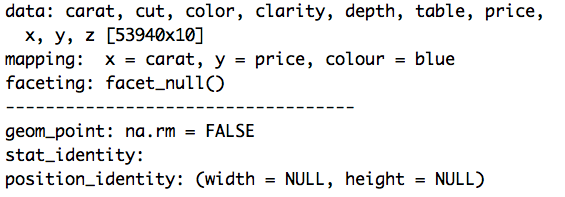
\includegraphics[width=110mm,scale=0.5]{bluemap.png}
\end{frame}


\begin{frame}\frametitle{How about blue points?}
\framesubtitle{Ahhhhh \ldots}
\footnotesize\texttt{p <- ggplot(data=diamonds, aes(carat, price)) + geom\_point(color = "blue")} 
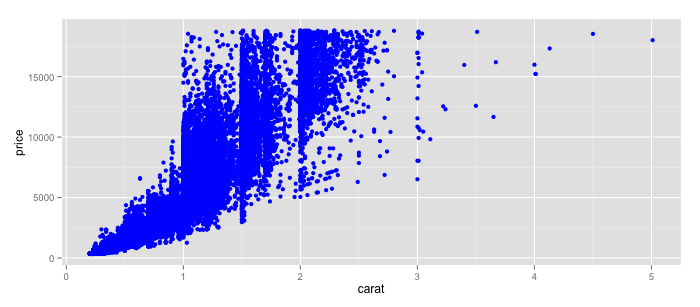
\includegraphics[width=100mm,scale=0.5]{qplotbluefixed.png}
\end{frame}

\begin{frame}\frametitle{Under the hood}
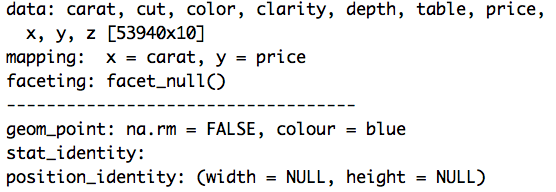
\includegraphics[width=110mm,scale=0.5]{bluemapcorrect.png}
\end{frame}


\begin{frame}\frametitle{How about a text annotation?}
\footnotesize\texttt{p <- ggplot(data=diamonds, aes(carat, price)) + geom\_point(color = "blue") +  geom\_text(data = diamonds, aes(.75, 15000), label = "Expensive")} 
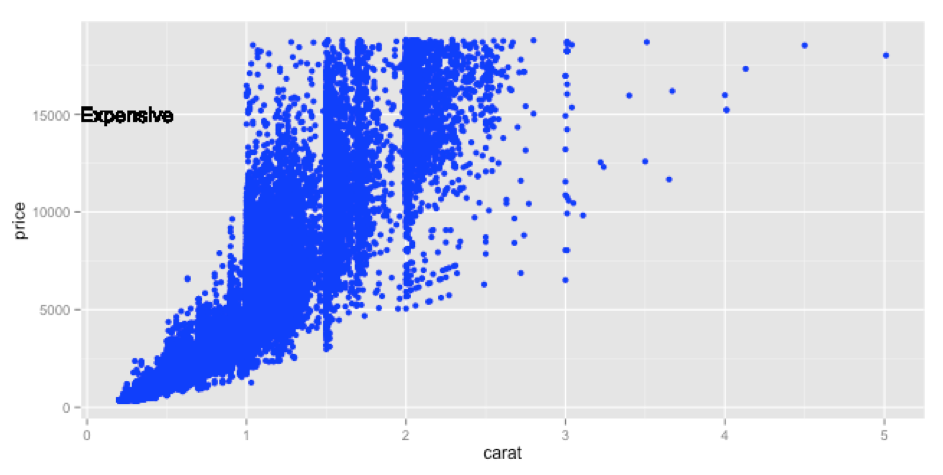
\includegraphics[width=100mm,scale=0.5]{wrongannotate.png} 
\alert{WTF?}
\end{frame}

\begin{frame}\frametitle{How about a text annotation?}
\framesubtitle{Ahhhhh \ldots}
\footnotesize\texttt{p <- ggplot(data=diamonds, aes(carat, price)) + geom\_point(color = "blue") + annotate("text", x = .27, y = 15000,label = "Expensive")} 
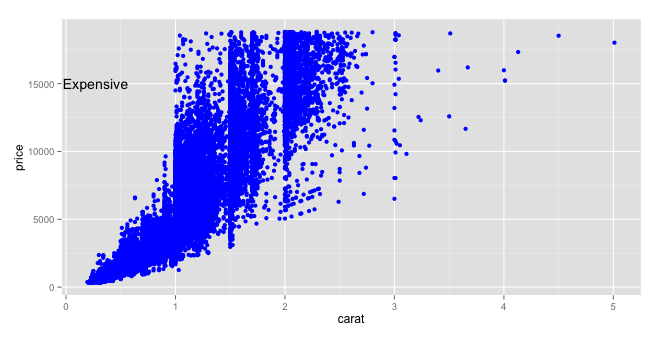
\includegraphics[width=100mm,scale=0.5]{rightannotate.png}
\end{frame}

\begin{frame}\frametitle{Under the hood}
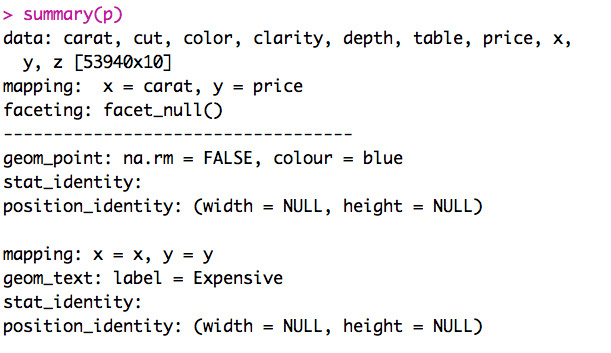
\includegraphics[width=110mm,scale=0.5]{hoodannotate.png}
\end{frame}






\begin{frame}
A few more examples \ldots
\end{frame}



\begin{frame}\frametitle{Worked example}
\framesubtitle{Overview of data}

	\begin{alertblock}{Science of science}
		\begin{itemize}
			\item Measurement of scientific growth 
			\item Co-authorship and network analysis
			\item Topic analysis
			\item Citation analysis
		\end{itemize}
	\end{alertblock}

	\begin{exampleblock}{Overview of data}
		\begin{itemize}
			\item Population set of social work journals ($N = 88$)
			\item Search of unique social science databases ($N = 35$)
			\item Retrieve all available article records in past 25 years ($N = 35k$)
		\end{itemize}
	\end{exampleblock}
\end{frame}




\begin{frame}
\footnotesize \texttt{minimal <- ggplot(author\_count, aes(pub\_year, paper\_percent, colour=n\_authors)) + 
  geom\_line()} 

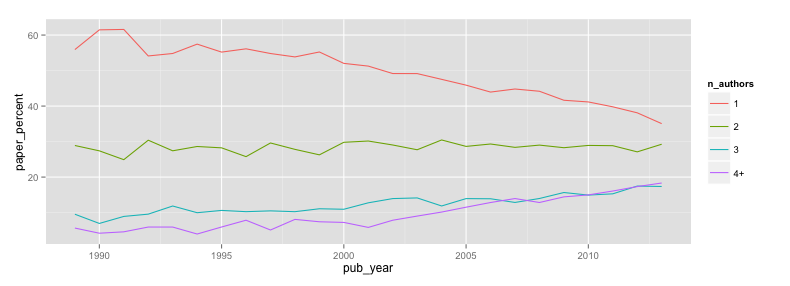
\includegraphics[width=110mm,scale=0.5]{minimal.png}
\end{frame}



\begin{frame}
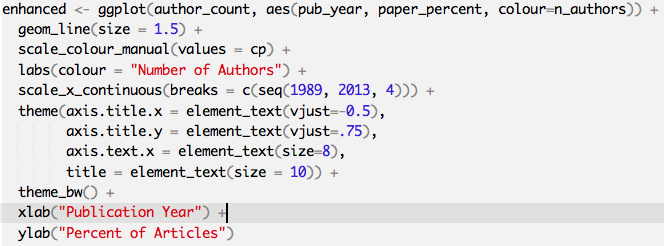
\includegraphics[width=110mm,scale=0.5]{enhancedcode.png}
\end{frame}

\begin{frame}
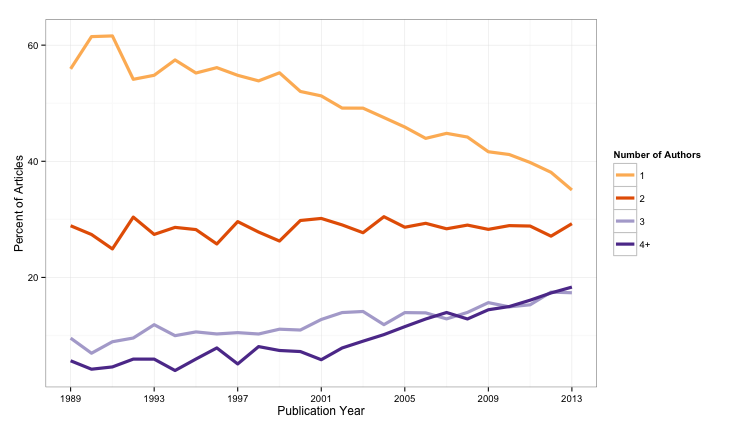
\includegraphics[width=110mm,scale=0.5]{enhanced.png}
\end{frame}



\begin{frame}
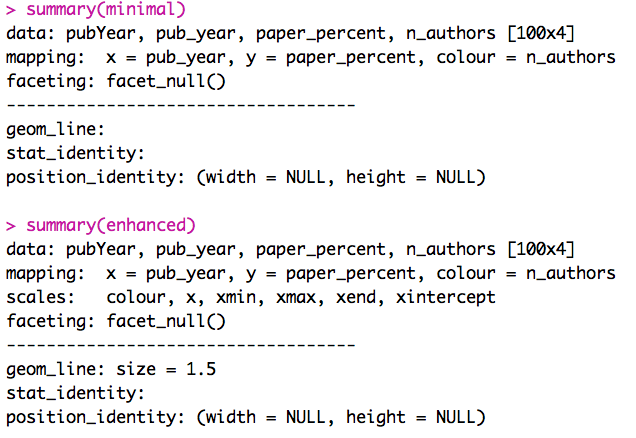
\includegraphics[width=90mm,scale=0.5]{authorhood.png}
\end{frame}


\begin{frame}
\footnotesize \texttt{facet\_plot <- ggplot(author\_count, aes(pub\_year, paper\_percent, colour=n\_authors)) + 
  geom\_line() + facet\_wrap($\sim$ journal)} 
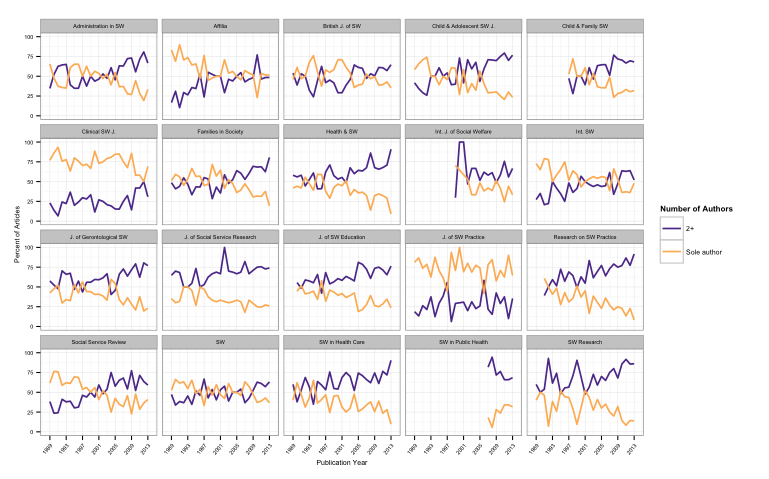
\includegraphics[width=110mm,scale=0.5]{facetplot.png}
\end{frame}



	



\end{document}